\documentclass[12pt,oneside]{book}
\usepackage{geometry}                		% See geometry.pdf to learn the layout options. There are lots.
\geometry{a4paper}                   			% ... or a4paper or a5paper or ... 
%\geometry{landscape}                		% Activate for for rotated page geometry
%\usepackage[parfill]{parskip}    		% Activate to begin paragraphs with an empty line rather than an indent
\usepackage{graphicx}				% Use pdf, png, jpg, or epsß with pdflatex; use eps in DVI mode
								% TeX will automatically convert eps --> pdf in pdflatex		
\usepackage{amssymb}

\usepackage[spanish]{babel}			% Permite que partes automáticas del documento aparezcan en castellano.
\usepackage[utf8]{inputenc}			% Permite escribir tildes y otros caracteres directamente en el .tex
\usepackage[T1]{fontenc}				% Asegura que el documento resultante use caracteres de una fuente apropiada.

\usepackage{hyperref}				% Permite poner urls y links dentro del documento

\title{Mi Juego Favorito}
\author{Javier Tibau}
%\date{}							% Activate to display a given date or no date

\begin{document}
\maketitle
\tableofcontents

\chapter{Introducción}
El libro a continuación es creado como una herramienta para el desarrollo de habilidades de edición colaborativa de documentos de texto plano. La herramienta que habilita dicha colaboración, en este taller, es Git pero podría ser reemplazada por otros sistemas de versionamiento.

\chapter{Los Juegos}

\section{Buscaminas}

\begin{figure}[htbp]
\begin{center}
\includegraphics[width=.60\textwidth]{./imagenes/minesweeper.png}
\caption{Buscaminas}
\label{Buscaminas}
\end{center}
\end{figure}
Buscaminas\footnote{\url{http://minesweeperonline.com/}} es uno de los juegos más jugados debido a lo ubicuo de su distribución. Fue incluido en 1992 en la versión de Windows 3.1 y desde entonces lo hemos encontrado presente en todas las versiones de dicho sistema operativo.
En la figura \ref{Buscaminas} puede ver una implementación web del juego.
La premisa del juego es simple: Limpiar el campo de juego sin hacer explotar ninguna de las minas que se encuentran en la cuadrícula.

\subsubsection{¿Por qué es uno de mis juegos favoritos?}
\begin{itemize}
\item[Javier Tibau] Las reglas del juego son sencillas y fáciles de entender. A pesar de esto, el juego no es atractivo para todo el mundo, creo que es un gusto adquirido. Las reglas me fueron presentadas por mi papá, quien en su máquina de trabajo con Windows 3.11 era uno de los pocos juegos ``divertidos'' que tenía. Para mi, el gran interés del juego es que destaca (o esconde) la resolución de problemas con fondo algebraico. En cierto momento del juego, y para el jugador que ha estudiado álgebra lineal, el reventar una casilla se torna similar a descifrar un sistema de ecuaciones con varias incógnitas. Los sistemas sencillos son bien definidos y tienen 2, 3 o hasta 4 incógnitas, mientras los más complejos pueden inclusive tener múltiples soluciones.
\end{itemize}

\section{Dota 2}

\begin{figure}[htbp]
\begin{center}
\includegraphics[width=.60\textwidth]{./imagenes/dota2.jpg}
\caption{Dota 2}
\label{Dota 2}
\end{center}
\end{figure}
Dota 2 \footnote{\url{http://dota2.com/}} es un juego creado por Valve basado en el popular mod de Warcraft 3, Defense of the Ancients. Es un juego de estrategia en equipo para ser jugado con equipos de 5 personas cada uno.
Dota 2 combina elementos de estrategia en tiempo real con perspectiva "en tercera persona", incorporando a todo ello un sistema de nivelación y jugabilidad de diversos juegos de rol como Diablo. Los jugadores asumen el papel de una unidad clasificado como un "héroe", que puede subir de nivel hasta un máximo de 25. La configuración básica de Dota 2 consiste en dos ciudades de distinta forma, cada una cuenta con una fortaleza de defensa conocida como "ancestro", situadas en los extremos opuestos de un mapa equilibrado de manera uniforme. Entre ellas hay varias regiones de conexión identificado como "caminos", que son atravesados por unidades enemigas, al tiempo que luchan contra poderosas torres defensivas a lo largo del camino. Los jugadores se dividen entre dos equipos, cada uno con hasta cinco jugadores, para competir como los principales defensores de cada Fortaleza de los Ancestros.

\subsubsection{¿Por qué es uno de mis juegos favoritos?}
\begin{itemize}
\item[Victor Cedeño] Este es un juego que requiere de comunicación y cooperación entre 5 personas para poder lograr el objetivo de vencer al otro equipo. Es muy dificil jugar solo sin la ayuda de tus compañeros. El juego tiene una gran selección de más de 100 heroes para elegir, esto quiere decir que cada partida es diferente ya que las combinaciones posibles de los equipos son innumerables. Es un juego que fomenta el trabajo en equipo y las decisiones correctas.
\end{itemize}

\include{juegos/Zelda}
\section{Sonic Generations}

Sonic Generations\footnote{\url{hwww.sega.com/sonicgenerations/‎} es un juego multiplataforma el cual ofrece una nueva experiencia en juego debido a que sus niveles son llevados a escenarios 2D y 3D recreando el ambiente del Sonic antiguo y del nuevo Sonic respectivamente. Este juego salió para PS3, Xbox360 y PC.
\section{Arcane Legends}

\begin{figure}[htbp]
\begin{center}
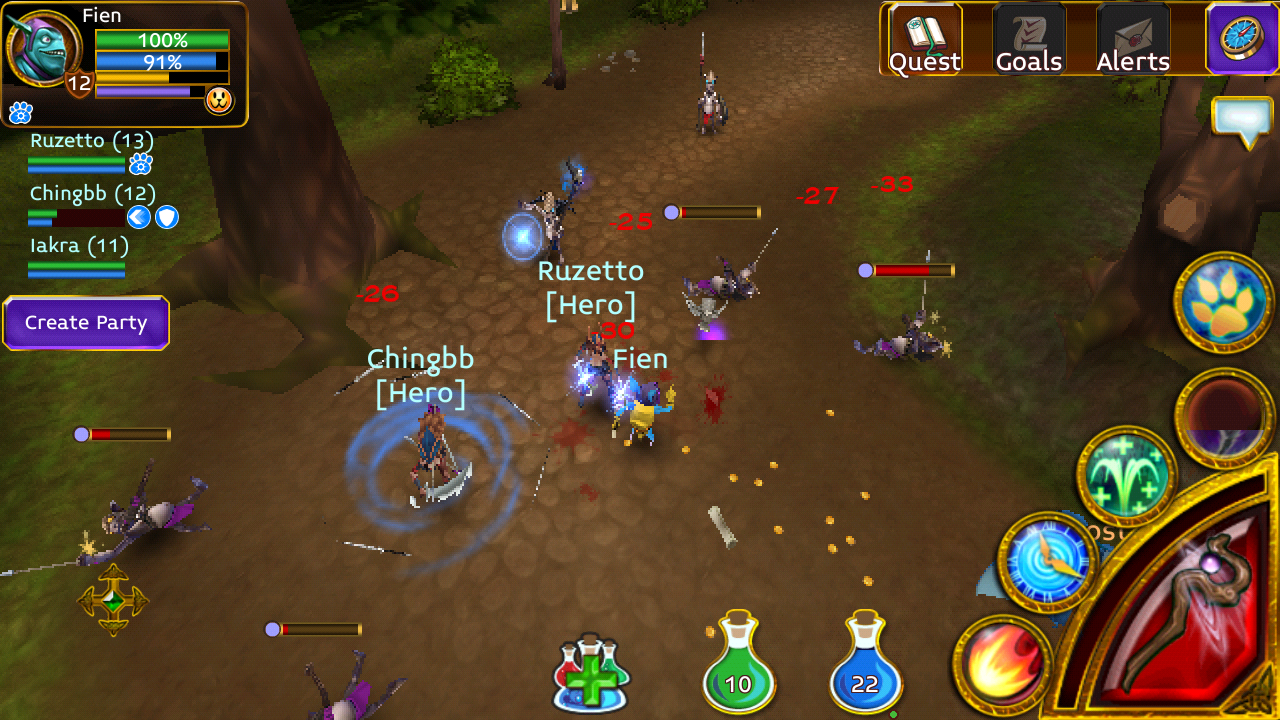
\includegraphics[width=.60\textwidth]{./imagenes/arcanelegends.png}
\caption{Arcane Legends}
\label{Arcane Legends}
\end{center}
\end{figure}
Arcane Legends\footnote{\url{http://www.arcanelegendsgame.com/}} es un juego para plataformas móviles de tipo MMORPG totalmente gratuito en el que podrás combatir en modo cooperativo con otros usuarios de la red y derrotar el mal que encontrarás por todas partes. El personaje que elijas marcará tu personalidad y puedes elegir tres tipos: un pícaro, un mago o un guerrero. Una de las mejores características del juego se basa en un compañero animal que llevas a tu lado y que podrás mandar a tu antojo para que te ayude en la lucha. Además podrás hacerle evolucionar y añadirle poderes extra.

\subsubsection{¿Por qué es uno de mis juegos favoritos?}
\begin{itemize}
\item[César Madrid]Arcane Legends en un juego que te ayuda a entretenerte en tus tiempos libres jugando con conocidos o descocidos a través de la red, en el cual puedes formar grupos para ir avanzando por nuevos mapas o puedes unirte a batallas de jugador contra jugador donde puedes ir demostrando tus habilidades con tu personaje y tu trabajo en equipo con el resto de tu grupo para así poder conseguir la victoria. Lo mejor de este juego es que aparte de jugarlo en tu pc a través de un navegador, también puedes jugarlo desde dispositivos móviles, como android e iOS, y así poder entretenerte en cualquier momento.
\end{itemize}

\section{Crysis 2}

\begin{figure}[htbp]
\begin{center}
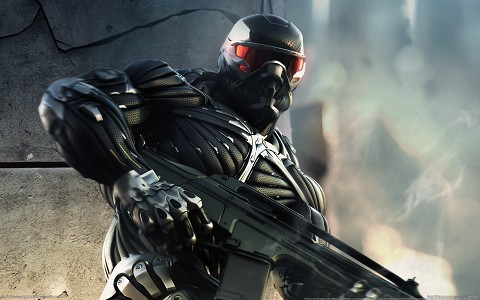
\includegraphics[width=.60\textwidth]{./imagenes/crysis2.jpg}
\caption{Crysis 2}
\label{Crysis 2}
\end{center}
\end{figure}
Crysis 2 \footnote{\url{http://www.ea.com/es/crysis2}} es un videojuego de disparos en primera persona desarrollado por la empresa Crytek y distribuido por Electronic Arts. Fue publicado en marzo del 2011 para PC, Xbox 360 y PlayStation 3. Es la secuela de Crysis y el primer videojuego en usar el motor CryEngine 3 desarrollado por Crytek también.

\subsubsection{¿Por qué es uno de mis juegos favoritos?}
\begin{itemize}
\item[Rubén Carvajal] La esencia del juego es magnífica, la historia consigue atraparte con su argumento futurístico.
Uno puede jugarlo a su manera, dependiendo del escenario habrán momentos en que te guste más pasar a todos descargando todo tu arsenal de armas, o momentos en que lo que sirva más sea utilizar las múltiples opciones del traje y el sigilo.
La jugabilidad y los gráficos son de altísima calidad, las opciones de camuflaje y el entorno en el que se desarrolla el juego son particularidades destacables.

El sonido de cada ambiente está bien trabajado, e incluso tenemos opciones gráficas en 3D, cosas que hacen de este un excelente juego.
\end{itemize}


\chapter{Conclusiones}
Cuales juegos fueron más populares y un breve razonamiento del porqué.

\end{document}  
